\subsection*{Problema 13}
\textbf{Enunciado:} Evaluar la integral definida 
$\int_{1}^{2} x^{-2} \, dx$ mediante sumas de Riemann.

\textbf{Solución:}
Para evaluar la integral definida mediante sumas de Riemann, utilizamos una partición en progresión geométrica del intervalo $[1, 2]$. 

Sea $n$ el número de subintervalos. Definimos la razón común de la progresión geométrica como:
\begin{align*}
q = 2^{1/n}
\end{align*}

Los puntos de la partición $P = \{x_0, x_1, \dots, x_n\}$ se definen como:
\begin{align*}
x_i = x_0 q^i = 1 \cdot (2^{1/n})^i = 2^{i/n}
\end{align*}
para $i = 0, 1, 2, \dots, n$. El ancho de cada subintervalo es:
\begin{align*}
\Delta x_i &= x_i - x_{i-1} \\
&= 2^{i/n} - 2^{(i-1)/n} \\
&= 2^{(i-1)/n}(2^{1/n} - 1)
\end{align*}

Tomamos el extremo izquierdo de cada subintervalo como punto muestra $x_i^* = x_{i-1} = 2^{(i-1)/n}$. La suma de Riemann se plantea como:
\begin{align*}
S_n &= \sum_{i=1}^{n} f(x_i^*) \Delta x_i \\
&= \sum_{i=1}^{n} \left(2^{(i-1)/n}\right)^{-2} \Delta x_i \\
&= \sum_{i=1}^{n} 2^{-2(i-1)/n} 2^{(i-1)/n}(2^{1/n} - 1)
\end{align*}

Simplificando los exponentes de base 2:
\begin{align*}
S_n &= (2^{1/n} - 1) \sum_{i=1}^{n} 2^{-(i-1)/n} \\
&= (2^{1/n} - 1) \sum_{j=0}^{n-1} \left(2^{-1/n}\right)^j
\end{align*}

La suma interior es una serie geométrica finita de razón $r = 2^{-1/n}$ y $n$ términos:
\begin{align*}
\sum_{j=0}^{n-1} r^j = \dfrac{1 - r^n}{1 - r} = \dfrac{1 - (2^{-1/n})^n}{1 - 2^{-1/n}} = \dfrac{1 - 2^{-1}}{1 - 2^{-1/n}}
\end{align*}

Sustituyendo este resultado en $S_n$:
\begin{align*}
S_n &= (2^{1/n} - 1) \left( \dfrac{1 - 1/2}{1 - 2^{-1/n}} \right) \\
&= (2^{1/n} - 1) \left( \dfrac{1/2}{1 - 2^{-1/n}} \right)
\end{align*}

Multiplicando numerador y denominador por $2^{1/n}$:
\begin{align*}
S_n &= \dfrac{2^{1/n} - 1}{2(2^{1/n} - 1) 2^{-1/n}} \\
&= \dfrac{2^{1/n}}{2} = \dfrac{2^{1/n}}{2^1} = 2^{(1/n) - 1}
\end{align*}

Finalmente, calculamos el límite cuando $n \to \infty$:
\begin{align*}
\int_{1}^{2} x^{-2} \, dx &= \lim_{n \to \infty} S_n \\
&= \lim_{n \to \infty} 2^{(1/n) - 1} \\
&= 2^{0 - 1} = 2^{-1} = \dfrac{1}{2}
\end{align*}

\begin{figure}[H]
	\centering
	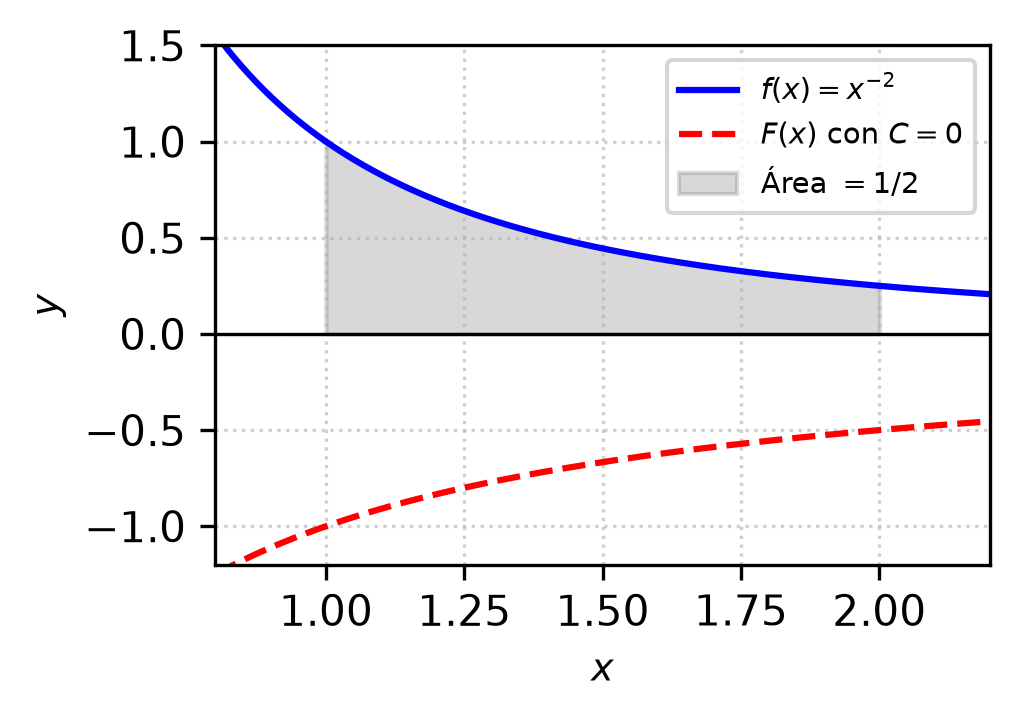
\includegraphics[width=\columnwidth]{semana_06/graficas/SEM06_P13_grafica.png}
	\caption{Representación gráfica de $f(x)$ y su antiderivada $F(x)$ evaluada para la constante de integración $C = 0$ (Problema 13).}
	\label{fig:problema13}
\end{figure}
